\section{Previous work} \label{tex:previous_work}


Ever since Rigamonti et al. in 2015\cite{Sironi2015} found that filters can be computed as a linear combination of smaller separable filters, many approaches have been considered using this principle in different ways. A filter is called separable when it can be expressed using multiple parts of lower dimension, as for instance using the CP-decomposition as they have illustrated in \autoref{fig:separable_filters}. 

\begin{figure}[ht]
    \centering
    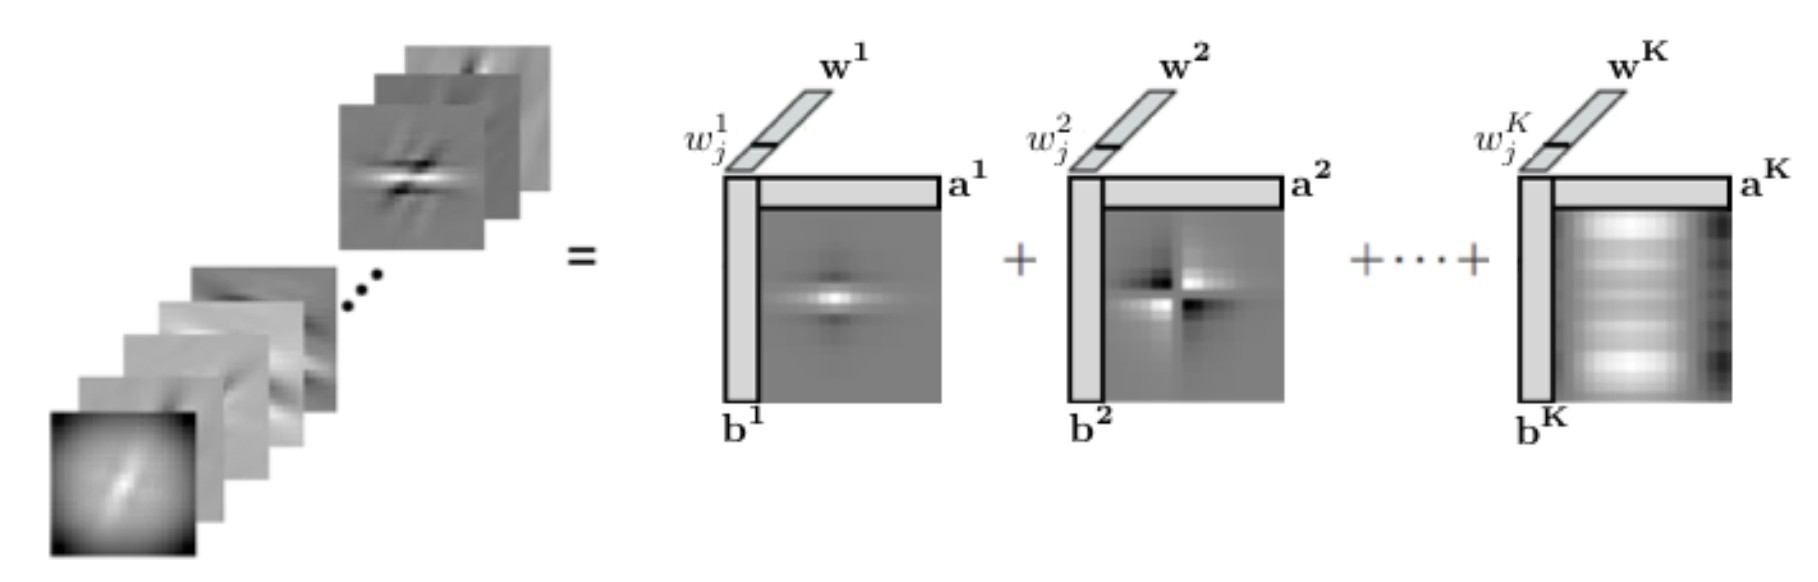
\includegraphics[width=.8\linewidth]{Pics/02_Previous_work/separable_filters.png}
    \caption{Taken from \cite{Sironi2015}. Left: A bank of two-dimensional filters is stacked together to form a 3-dimensional tensor. Right: The tensor is decomposed in the sum of K rank-one tensors. Thus, the original filters are approximated by the weighted sum of the separable filters $s_k = \boldsymbol{a}_k \circ \boldsymbol{b}_k$}
    \label{fig:separable_filters}
\end{figure}

